\section{Results and Discussions}

\begin{figure}[ht]
    \centering
    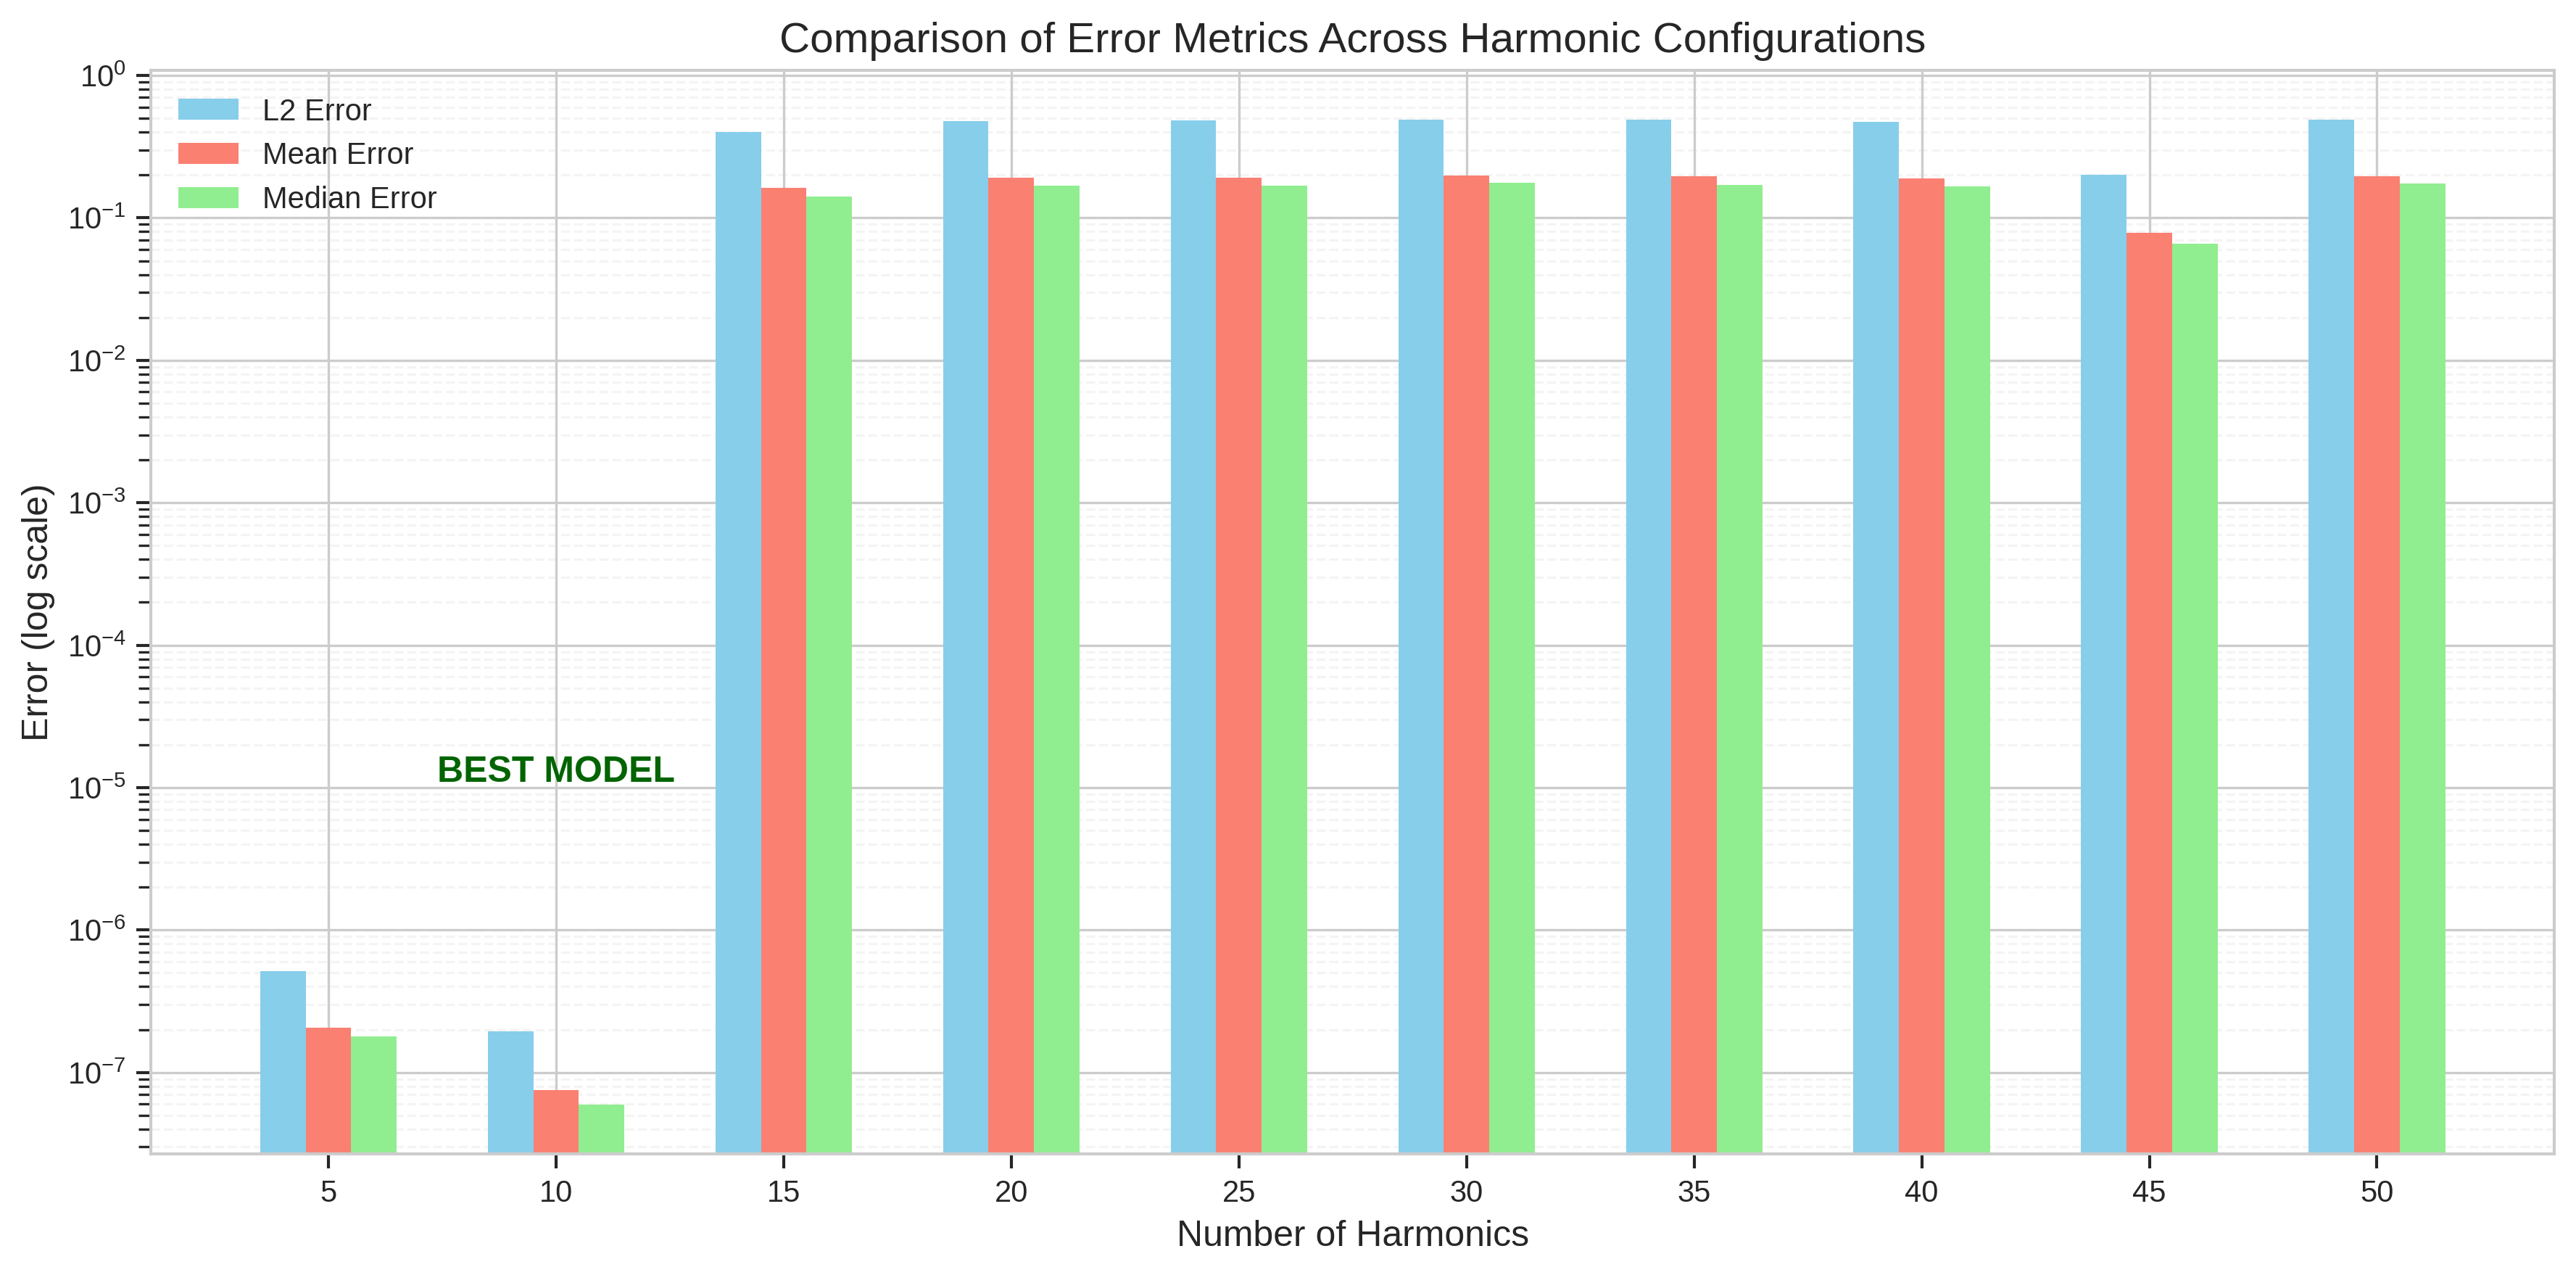
\includegraphics[width = 1.0\linewidth]{figures/error_metrics_comparison.png}
    \caption{Comparison of error metrics across different harmonic configurations. The plot demonstrates the non-monotonic relationship between harmonic count and solution accuracy, with the optimal performance achieved at 10 harmonics.}
    \label{fig:error_metrics}
\end{figure}


\begin{table}[ht]
    \centering
    \caption{Performance metrics for different harmonic configurations, highlighting the optimal performance at 10 harmonics}
    \label{tab:harmonic_comparison}
    \begin{tabular}{|c|c|c|c|c|}
    \hline
    \textbf{Harmonics} & \textbf{L2 Error} & \textbf{Max Error} & \textbf{Mean Error} & \textbf{Median Error} \\ \hline
    5    & $5.12 \times 10^{-7}$ & $5.36 \times 10^{-7}$ & $2.07 \times 10^{-7}$ & $1.79 \times 10^{-7}$ \\ \hline
    10   & $\mathbf{1.94 \times 10^{-7}}$ & $\mathbf{3.58 \times 10^{-7}}$ & $\mathbf{7.50 \times 10^{-8}}$ & $\mathbf{5.96 \times 10^{-8}}$ \\ \hline
    15   & $4.02 \times 10^{-1}$ & $4.95 \times 10^{-1}$ & $1.62 \times 10^{-1}$ & $1.42 \times 10^{-1}$ \\ \hline
    20   & $4.80 \times 10^{-1}$ & $4.92 \times 10^{-1}$ & $1.92 \times 10^{-1}$ & $1.68 \times 10^{-1}$ \\ \hline
    30   & $4.92 \times 10^{-1}$ & $4.98 \times 10^{-1}$ & $1.98 \times 10^{-1}$ & $1.77 \times 10^{-1}$ \\ \hline
    45   & $2.00 \times 10^{-1}$ & $3.39 \times 10^{-1}$ & $7.84 \times 10^{-2}$ & $6.61 \times 10^{-2}$ \\ \hline
    \end{tabular}
\end{table}
